\documentclass[a4paper]{jpconf}
\usepackage{graphicx}
\usepackage{color}
\usepackage{array}
\usepackage{enumerate}

\begin{document}
\title{WLCG and IPv6 - the HEPiX IPv6 working group}

\author{S Campana$^1$, K Chadwick$^2$, G Chen$^3$, J Chudoba$^4$, P Clarke$^5$, M Eli\'a\v s$^4$,
        A Elwell$^1$, S Fayer$^6$, T Finnern$^7$, L Goossens$^1$,
        C Grigoras$^1$, B Hoeft$^8$, D P Kelsey$^9$, T Kouba$^4$, 
        F L\'opez Mu\~noz$^{10}$, E Martelli$^1$, M Mitchell$^{11}$, A Nairz$^1$, 
        K Ohrenberg$^7$, A Pfeiffer$^1$, F Prelz$^{12}$, F Qi$^3$, D Rand$^6$, 
        M Reale$^{13}$, S Rozsa$^{14}$, A Sciab\`a$^1$, R Voicu$^{14}$, 
        C J Walker$^{15}$ and T Wildish$^{16}$}

\address{$^1$ CERN, CH-1211 Gen\`eve 23, Switzerland}
\address{$^2$ Fermi National Accelerator Laboratory, Batavia, Il 60510, U.S.A.}
\address{$^3$ Institute of High Energy Physics, 19B Yuquanlu, Shijingshan District, 100049 Beijing, China} 
\address{$^4$ Institute of Physics, Academy of Sciences of the Czech Republic Na Slovance 2 182 21 Prague 8, Czech Republic}
\address{$^5$ The University of Edinburgh, Mayfield Road, Edinburgh EH9 3JZ, United Kingdom}
\address{$^6$ Imperial College London, South Kensington Campus, London SW7 2AZ, United Kingdom}
\address{$^7$ Deutsches Elektronen-Synchrotron, Notkestra\ss e 85, D-22607 Hamburg, Germany}
\address{$^8$ Karlsruher Institut f\"ur Technologie, Hermann-von-Helmholtz-Platz 1, D-76344 Eggenstein-Leopoldshafen, Germany}
\address{$^9$ STFC Rutherford Appleton Laboratory, Harwell Oxford, Didcot, Oxfordshire OX11 0QX, United Kingdom}
\address{$^{10}$ Port d'Informaci\'o Cient\'ifica, Campus UAB, Edifici D, E-08193 Bellaterra, Spain}
\address{$^{11}$ University of Glasgow, Kelvin Building, University Avenue, Glasgow G12 8QQ, United Kingdom}
\address{$^{12}$ INFN, Sezione di Milano, via G. Celoria 16, I-20133 Milano, Italy}
\address{$^{13}$ Consortium GARR, Via dei Tizii 6, I-00185 Roma, Italy}
\address{$^{14}$ California Institute of Technology, Pasadena, Ca 91125, U.S.A.}
\address{$^{15}$ Queen Mary University of London, Mile End Road, London E1 4NS, United Kingdom}
\address{$^{16}$ Princeton University, Jadwin Hall, Princeton, NJ 08544, U.S.A.}

\ead{david.kelsey@stfc.ac.uk, ipv6@hepix.org}

\begin{abstract}
The HEPiX ({\tt http://www.hepix.org}) IPv6 Working Group has 
been investigating the many issues which feed into the decision on the 
timetable for the use of IPv6 ({\tt http://www.ietf.org/rfc/rfc2460.txt}) 
networking protocols in High Energy Physics (HEP) Computing, in
particular in the Worldwide Large Hadron Collider (LHC) Computing Grid (WLCG).
RIPE NCC, the European Regional Internet Registry (RIR), ran 
out of IPv4 addresses in September 2012. The North and South America RIRs 
are expected to run out soon. In recent months it has become more clear 
that some WLCG sites, including CERN, are running short of IPv4 address space, 
now without the possibility of applying for more. This has increased the 
urgency for the switch-on of dual-stack IPv4/IPv6 on all outward facing WLCG 
services to allow for the eventual support of IPv6-only clients. The 
activities of the group include the analysis and testing of the readiness 
for IPv6 and the performance of many required components, including the 
applications, middleware, management and monitoring tools essential for 
HEP computing. Many WLCG Tier 1/2 sites are participants in the
group's distributed IPv6 testbed and the major LHC
experiment collaborations 
are engaged in the testing.  We are constructing a group 
web/wiki which will contain useful information on the IPv6 
readiness of the various software components and a knowledge base
({\tt http://hepix-ipv6.web.cern.ch/knowledge-base}).
This paper describes the work done by the working group and its future plans.
\end{abstract}

\section{Introduction}
%section 1

Blah blah management board timeline.


%\section{IPv6: the general problem}
\section{IPv6: the general problem}

The intention of the designers of the IPv6 protocol was to make it full of appealing features, in order to push its adoption widely and quickly. 
The IPv6 specifications (RFC 1883/RFC 2460) \cite{rfc}
were set back in 1995, when the Internet community realized that the classful allocation policies of the time were causing a quick depletion of the address space. 
\par
Unfortunately for IPv6, the IPv4 problem was quickly fixed with the adoption of the classless allocations (CIDR, RFC 1519 \cite{rfc}) and by the invention of Address and Port translation techniques (NAT, RFC 1631 \cite{rfc}). These events, together with the fact that the IPv6 advantages were far less appealing than the cost of deploying it, put the protocol in a limbo where it stayed for almost twenty years, until IPv4 addresses became scarce again.
\par
At the end of the first decade of the 21st century, the RIRs started warning the Internet community that IPv4 addresses would soon be exhausted and urged everyone to adopt IPv6. IPv6 was quite quickly deployed on the Internet backbones, but not where it would have brought the most of its benefits, at the client and content side. 
Plagued by the chicken and the egg problem (no users if no content, no content if no users), in 2012 finally some of the 
biggest content providers made the bold move to make their services available over IPv6. 
One year later, the IPv6 global traffic is gradually increasing but still counts as a very small fraction of the 
total Internet traffic \cite{ipv6stat}.

\section{IPv6 at CERN}
Many academic institutions, which joined the Internet when it was in a very early stage, are still enjoying the large allocations that were given in those days; thus they are lacking of any urge to move to IPv6.
\par 
This was the situation at CERN till 2011, when Server Virtualization started being used. The virtualization technique proved to be very effective and its adoption at CERN has grown exponentially. In 2012, when the plan for the services to be run in the upcoming remote data centre in Wigner (Budapest, HU) was finalized, it became clear that something like 250,000 public IP addresses would be needed in the near future. At the same time, RIPE, the European Internet Registry, was announcing the adoption of a new conservative allocation policy that would grant no more than 1024 IPv4 addresses to any requester. 
It could have been an impasse for the IT deployment plans, but luckily CERN had been testing with IPv6 since 1998 and in 2011 the management of the IT department approved the project to deploy IPv6 in the CERN campus and datacentres, when its need had yet to be proven.
\par
For large enterprises like CERN, deploying IPv6 is not as simple as configuring a dozen routers to be dual stack. The Network Management System and the Network database had to be made IPv6 aware, all the IPv6 information generated and all the basic network services configured: the Domain Name Service (DNS), the Network Time Protocol (NTP), the Dynamic Host Configuration Protocol (DHCPv6), etc. 
At the same time the network security had to be kept at the same level as always.
After two years, the deployment is almost completed; right in time to tackle the IPv4 exhaustion problem that most likely will hit CERN in 2015 when the Wigner datacentre will reach its full capacity. 
Many applications still cannot make use of IPv6, thus it is very premature to deploy IPv6-only Virtual Servers. The strategy will be to deploy a hybrid solution where servers get a private IPv4 address and a public IPv6 one. The private IPv4 address will allow legacy applications to work within the CERN domain,  while the public IPv6 address will allow world-wide reachability.
\par
Hopefully the availability of LHC data over IPv6 will push IPv6 adoption in the large WLCG community.


\section{The HEPiX IPv6 working group}
The HEPiX forum brings together worldwide IT staff, including system administrators, system engineers, and managers from the HEP and Nuclear Physics laboratories and institutes, to foster a learning and sharing experience between sites facing scientific computing and data challenges. At its semi-annual meetings, HEPiX had been considering the issue of migration to IPv6 for a number of years. At the end of 2010 a survey of HEP sites around the world was made asking about their plans for the deployment of IPv6. While it was very clear that there was no requirement for an urgent move to IPv6 a good number of sites were planning such a deployment and a few, particularly CERN, reported a foreseen lack of IPv4 address space in the not too distant future.

It was realised that any decision to deploy IPv6 on the WLCG infrastructure would involve much testing and planning and the decision was therefore taken to start a dedicated working group to investigate the issues. The HEPiX IPv6 working group was formed in 2011 with the following mandate.

Phase 1 of the work was to consider whether and how IPv6 should be deployed in HEP (especially for WLCG). This involved:
\begin {itemize}
\item A Readiness and Gap analysis
\item The need to include all relevant HEP applications, middleware, security issues, system management and monitoring tools, and end-to-end network monitoring
\item Running a distributed HEPiX IPv6 testbed to explore all of the above issues
\item An initial report at the end of 2011
\end {itemize}	
Following that initial report it was agreed that the work should continue and that phase 2 of the work should include:
\begin {itemize}
\item The proposal of a timetable and an analysis of the resources required for the deployment of IPv6 on WLCG
\item The production of an implementation plan including advice to HEP sites on deployment
\end {itemize}

Since then the group has been working on the mandated tasks and meeting regularly with quarterly face to face meetings at CERN and monthly video/phone meetings to review progress. Full details are available at {\tt http://indico.cern.ch/categoryDisplay.py?categId=3538}.




\section{The IPv6 testbed}
The impact of IPv6 is not limited to the transport layer 
but introduces the need for choice and preference in name-to-address 
resolution, implies multi-homing of all network endpoints (possibly on 
multiple protocol versions) and requires opaque handling of address 
information. This broadens the scope of code changes needed to add
IPv6 support to existing code and adds to the complexity of testing:
continued operation on IPv4 on dual-stack hosts, then preference of IPv6 and 
options to control it for all network bindings and connections
need to be verified with adequate code coverage.
\par
At opposite ends of the spectrum of practical testing options are
testing of individual, isolated components and services and the analysis of 
integrated services on dual-stack nodes. Both approaches are incomplete:
\begin{itemize}
\item[-] testing of isolated components misses the interaction with other
services at the OS level and usually requires services to be configured
differently than for production;
\item[-] testing of production-ready, integrated nodes may just be 
accidentally focusing on normal operation and bring insufficient 
code and functionality coverage.
\end{itemize}
This calls for a complementary approach,
where individual services are deployed and tested within the scale of
available dedicated resources and, once sufficient confidence and knowledge
of their level and mode of IPv6 support is built, are watched in the context
of a production node with dual-stack network and dual IPv4/IPv6 public address
resolution.
\par
Desirable characteristics of a dedicated testbed for single-service testing are:
\begin{itemize}
\item Geographical spread covering all ranges of realistic network latencies
and as many network providers as possible.
\item Uniform authentication/authorization scheme to factor out AA issues.
\item Uniform OS installation, to factor out any issue with the custom 
configuration needed to test isolated services and for easier
deployment of new services.
\end{itemize}
The current list of active testbed nodes can be found at the following URL:\\
{\tt http://hepix-ipv6.web.cern.ch/testbed-nodes}\\
While we have at the time of writing a reasonable
9-site/6-National Research and Education Network (NREN) coverage of Europe, the only non-european sites in the testbed
are IHEP Beijing in China and Fermilab in the US. More testbed sites are both needed and welcome to join 
to achieve a better match of our stated testbed goals.
\par
As for OS distributions, testbed nodes are mostly installed with 
Scientific Linux (CERN) version 5,
to replicate production conditions at LCG Tier-X centres. A few testbed nodes
have Red Hat Enterprise Linux (RHEL) \cite{rhel} version 6 derivatives installed: this allowed us to discover 
(and document in our knowledge base, {\tt http://hepix-ipv6.web.cern.ch/knowledge-base})
that, rather unexpectedly, {\tt libc} on RHEL version 6 causes unspecified 
protocol sockets to be bound on IPv4 only, instead of dual-stack 
as it used to be.
\par
To achieve the simplest possible authentication scheme, a custom Globus
Security Infrastructure (GSI)
plug-in maps all members of our test Virtual Organisation (VO) ({\tt ipv6.hepix.org}) to one
local account, logging any access. 
\par
The first service we deployed for standalone testing through the testbed was
GridFTP (or, more accurately, {\tt gsiftp}). 
This was not only because of GridFTP's basic role in WLCG data
transfer, but also because the FTP protocol (the GSI extensions don't 
affect but also suffer from this issue) is a paradigmatic example of 
how non-trivial IPv6 support can be. The original FTP specifications 
(RFC 765/RFC 959 \cite{rfc}) used the quad-byte notation for IP addresses 
{\em in the syntax of the FTP protocol commands} {\tt PORT} and {\tt PASV}.
This required the introduction, with RFC 2428 (September 1998) \cite{rfc} of
``extended'' versions of the same commands, supporting different address
families, and IPv6 in particular. We found on our testbed that support for 
the 'extended' command forms (and thus {\em implicitly} for IPv6)
is missing from certain FTP client implementations. Retrofitting the
clients with these commands is definitely more than a simple change in
the transport layer and serves as an example of how ramified the
introduction of 'IPv6 support' can be.
\par
Building on this mesh of GridFTP servers, both continuous direct point-to-point 
file transfer tests and tests of the File Transfer Service 
(FTS), were successfully carried out. Storage Resource Manager (SRM) endpoints
were also added, as described in detail in the next section.


\section{IPv6 testing and results}
\subsection{Testing scenarios}
In order to prepare the WLCG infrastructure for IPv6, the best
approach is to identify beforehand the relevant use cases, starting
from the simplest ones, to take into account the likely constraints
from sites and finally to define realistic scenarios to be used for
testing.

It is reasonable to assume that all central services must work in
dual-stack mode, to be compatible with both IPv4 and IPv6
clients. Site services are strongly encouraged to be run in dual stack
mode as well, lest they incur in limitations (for example in joining
storage federations). On the other hand, clients (including users,
software agents and jobs running on worker nodes) should be able to
exclusively use either protocol: users may connect from arbitrary
nodes (e.g. their laptops) while compute nodes at some sites might have
only IPv6 public addresses.

To summarise, any testing should comply with these requirements:
\begin{itemize}
\item all services must be tested in dual stack
\item all user clients must be tested in IPv4 and dual stack
\item all batch nodes must be tested in IPv4, IPv6 and dual stack (not all configurations might be possible for a given site)
\end{itemize}

The use cases to test are of increasing complexity and should be addressed in this order:
\begin{enumerate}[a.]
\item basic job submission, either direct (via CREAM client \cite{cream}, Condor-G, etc.) or via workload management services (EMI WMS \cite{wms}, glideinWMS, PanDA \cite{panda}, etc.)
\item basic data transfer from/to a user node to/from a storage element
\item third party data transfer (e.g. via FTS \cite{fts})
\item production data transfer (e.g. via PhEDEX \cite{phedgen}, DIRAC, etc.)
\item conditions data access (e.g. via Frontier/squid)
\item experiment software access (e.g. via CVMFS \cite{cvmfs})
\item experiment workflow, running a complete production/analysis task
\item information system query (e.g. via BDII \cite{bdii})
\item job monitoring (e.g. via MonALISA \cite{monalisa}, experiment dashboards, etc.)
\end{enumerate}
In all cases, all relevant client/service combinations in terms of network protocols should be addressed. For simplicity, ``auxiliary'' services (ARGUS, VOMS, MYProxy, etc.) running only IPv4 may be used.


\subsection{Point-to-point testing}

We used the PhEDEx LifeCycle agent \cite{LifeCycle} to drive transfers between pairs of sites, using gridftp with the IPv6 connectivity flags. Filesizes were checked at the destination, and any failures recorded. Files were transferred in both directions between each site pair.

Initially, we simply tested connectivity and basic functionality. We also tested under specific conditions, e.g. to compare throughput and error rates with IPv6 vs. IPv4 connectivity. This was useful for debugging issues with firewalls, etc.

Since March 2013 the transfer testbed is running continuously, with more sites joining over time. Finally we have 12 sites transferring 1 GB files among each other.

To date, we have transferred over 2 PB of data between the 12 sites over the 6 months since the testbed started continuous operations. This is 7\% of the rate that CMS \cite{cms} achieve in daily operations, so is quite significant. The average success rate is 87\%, which is very high considering that the testbed is operated at-risk. Errors are only detected when someone decides to look for them, and were often left unfixed to aid debugging.
So we can conclude that gridftp transfers over IPv6 are very reliable, given adequate hardware to run on.

Figure \ref{fig:full-mesh} shows transfer results for the full mesh of sites. The source site is shown along the rows, the destination site is shown in the columns. All plots are scaled to an x-axis of 500 seconds (corresponding to a transfer rate of 2 MB/sec), and only successful transfers are shown.

We can see that, in general, transfers were fast, the graphs mostly peak to the left. Some sites (IHEP Beijing, Chicago) have long tails for transfers out, though transfers to them are more successful.

\subsection{Testing with PhEDEx transfers}
We also tested with PhEDEx \cite{PhEDEx}, the CMS data-placement system. We used two WLCG/GridPP sites (Imperial College London and Glasgow) with IPv6-enabled Disk Pool Manager (DPM) storage elements, and transfers via a dual-stack FTS3 \cite{FTS3} server at Imperial College. Transfers were throttled to limit the load on the servers, and have been running smoothly for nearly two months at the time of writing, transferring over 120 TB of data. This tells us that PhEDEx can indeed operate to CMS production standards with IPv6-enabled services.
% Figure \ref{fig:phedex-transfer-volume} shows the accumulated volume of data transferred from mid-August until early October 2013, by which point over 120 TB of data had been transferred with very few errors. This tells us that PhEDEx can indeed operate to CMS production standards with IPv6-enabled services.

% To create this graphic:
% 1) save your image as a 1024x1024 png/gif/bmp
% 2) convert to pdf (install ImageMagick, then 'convert FileIn.png FileOut.pdf')
% 3) to resize the image, if needed, 'convert FileIn.png -resize 66% FileOut.pdf' etc
% N.B. if the input and output files have the same base name, LaTeX will prefer to take the png
% over the pdf, which is probably not what you want. Make sure the files have different names!
\begin{figure}[htp]
\centering
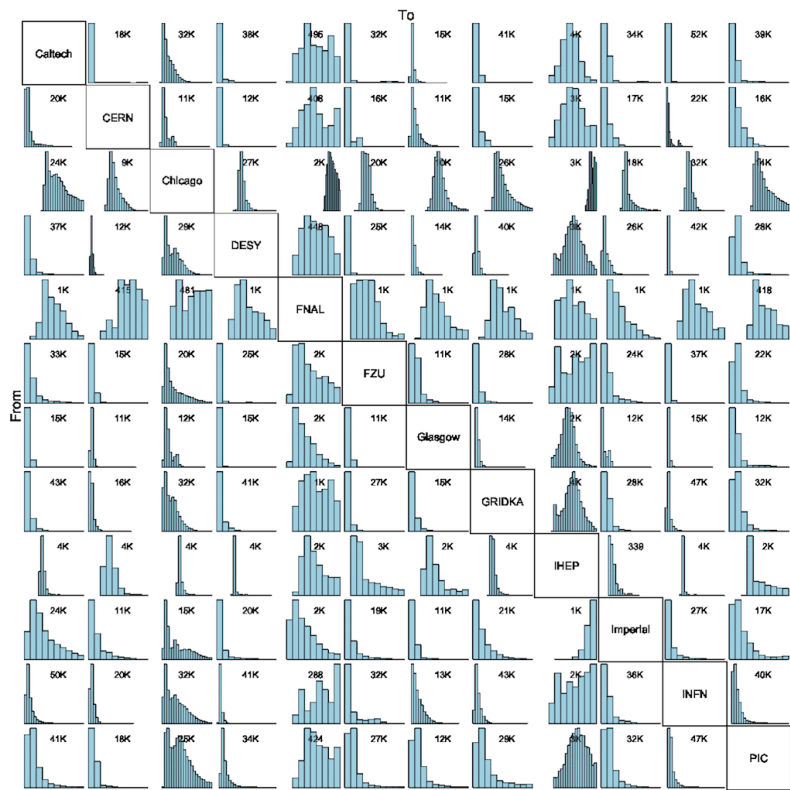
\includegraphics{full-mesh}
\caption{Transfer performance for the IPv6 testbed continuous transfers. A 1 GB file is transferred between each pair of sites, then deleted, then transferred again, continuously. The plots show the distribution of transfer duration times per site pair. The source site is named in the row, the destination site is named in the column. So the top-right plot shows transfers from Caltech to PIC, the bottom-left shows transfers from PIC to Caltech. The x-axis is in seconds, from 0 to 500 for each plot. The number inset in each plot shows the approximate number of transfers between that site pair in that direction.}\label{fig:full-mesh}
\end{figure}

%\begin{figure}[htp]
%\centering
%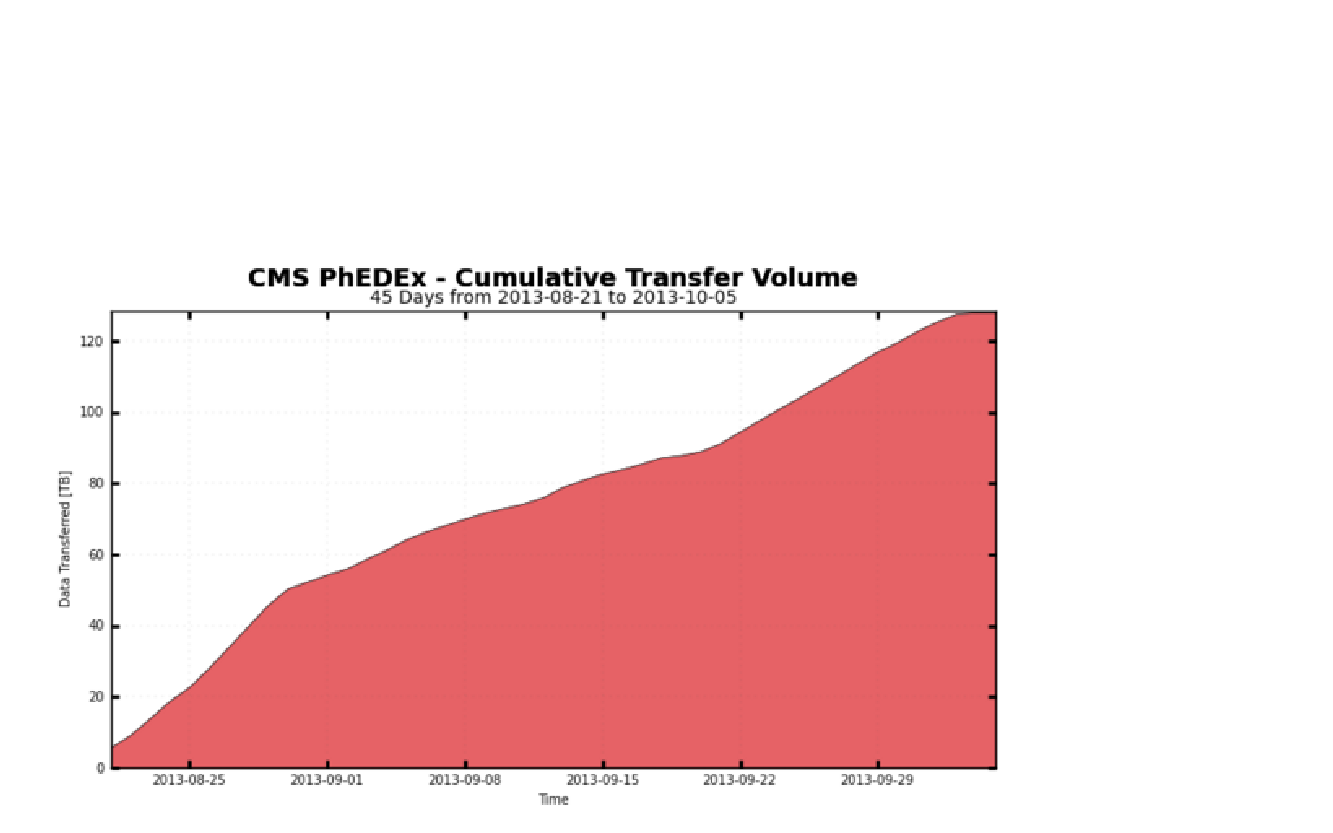
\includegraphics{phedex-transfer-volume}
%\caption{Cumulative data-transfer between Imperial College and Glasgow using PhEDEx on the IPv6 testbed.}\label{fig:phedex-transfer-volume}
%\end{figure}

\subsection{Dual-stack hosts at Imperial College London}
The WLCG/GridPP site within the HEP group at Imperial College London (UKI-LT2-IC-HEP) has configured a subset of its hosts to be dual-stack. 
The site currently runs dual-stack DNS, SSH, NFS, EMI 2 and EMI 3 CREAM CEs, EMI 2 Worker Nodes, 
ARC CE and dCache (headnode, SRM component only) services.
Additionally, all BDII services including top and site BDIIs run in dual-stack mode. The Puppet configuration system and the local OS install system have been left IPv4-only.
This set up was achieved in a number of stages. Initially, the local campus network team enabled 
stateless address autoconfiguration (SLAAC) on the subnet routers servicing the grid hosts. {\em All hosts} acquired an IPv6 address via autoconfiguration. 
No subsequent problems were observed and no hosts required IPv6 to be turned off in order to continue normal operations. 
Next, AAAA records were added to core services such as mail and LDAP. The DNS servers had static IPv6 addresses added. 
The IPv6 DNS server hostnames were added into {\tt /etc/resolv.conf} on all hosts. AAAA and PTR records were added to the worker nodes and these were made to point to the SLAAC addresses. 
On relevant service hosts the IPv6 firewall was configured as appropriate. On hosts running a BDII service the IPv6 option was enabled explicitly 
(by setting {\tt BDII\_IPV6\_SUPPORT=yes} in {\tt /etc/sysconfig/bdii}).


\section{Software and tools survey}
For a successful transition to the use of IPv6 it is necessary to do a full survey of all important applications, middleware and operational tools. We decided to focus on the IPv6 readiness of the important WLCG outward-facing services and all essential applications and management and monitoring tools. We have created an online database of IPv6-readiness where for each software component considered we can store its known state of readiness and details of any testing performed by us or others.

IPv6-readiness is not a simple yes/no question. There are various stages of readiness to be addressed.
Does the service break/slow down when used with IPv4 on a dual-stack host with IPv6 enabled?
Will the service try using (connecting/binding to) an IPv6 address (AAAA record), when available from DNS?
Will the service prefer IPv6 addresses from DNS, when preferred at the host level?
Does this need to be configured and how?
Can the service be persuaded to fall back on IPv4 if needed?
In many ways the most important question is the first one. As long as a service deployed on a dual-stack host behaves properly for IPv4 then we are safe to recommend such a deployment on the WLCG production infrastructure.
The current state of our survey may be seen at
{\tt http://hepix-ipv6.web.cern.ch/wlcg-applications}.

At the time of 
writing, there are still many packages which need further investigation and testing. Software known not to be ready for IPv6 at this time includes OpenAFS servers and clients, all but the latest release of dCache and many batch systems. Full details of all such problems and investigations will be recorded in our online database.




%\section{Collaboration with other groups}
%blah blah


\section{Outlook and future plans}
The IPv6 working group has made good progress but has to date only tested a small fraction of the many 
software components required by WLCG. There are still many more tests and 
assessments to be made and advice on dual-stack deployment to be formulated before 
our work can in any way be defined as complete.

Testing will continue in three areas. Firstly we will continue the mesh of data transfer tests between
the testbed sites, expanding to include new types of storage element and allowing for the ongoing
assessment of reliability. Some testbed sites are now working on the deployment of larger scale IPv6 testbeds
to allow the testing of IPv6-readiness in a more realistic production environment. Finally, we will encourage 
more Tier 2 sites to repeat the
tests at Imperial College (see section 6.4) by enabling dual-stack services on some or all of their production
services. Across all of these different scenarios we will gradually work through the list of testing scenarios presented
in section 6.1 together with representatives of the experiments.  During all of this testing we
will continue to update our online database with the details of IPv6 readiness.

At the time of our status report to HEPiX and the WLCG Management Board in 2012 we concluded that
the support of IPv6-only clients on WLCG was unlikely to be possible before January 2014. At the time of writing this is still true and indeed it is now clear that it will take much longer. Not only does the working group still have many tests to perform
but all of the many Tier 1 and Tier 2 sites need to complete the deployment of an IPv6 infrastructure at their site. This needs to include
the revision of local procedures and management tools and the provision of adequate training for network,
system operations and security staff. Once we have achieved this we can propose a more general deployment of 
production-level dual stack services thereby allowing for the eventual support of IPv6-only clients on WLCG.


\par
\section*{References}

\begin{thebibliography}{1}
\bibitem{ipv6wg} {\tt http://hepix-ipv6.web.cern.ch}
\bibitem{rfc} All Internet Engineering Task Force Requests For Comments (RFC) documents are available
from URLs such as http://www.ietf.org/rfc/rfcNNNN.txt where NNNN is the RFC number, for example {\tt http://www.ietf.org/rfc/rfc2460.txt}
\bibitem{planningguides} There is abundant refernce material at
{\tt http://www.internetsociety.org/deploy360/resources/ipv6-address-planning-guidelines-for-ipv6-address-allocation/} and {\tt https://www.ripe.net/support/training/material/IPv6-for-LIRs-Training-Course/Preparing-an-IPv6-Addressing-Plan.pdf}.
\bibitem{CiscoBook}
    Hogg S, Vyncke E - IPv6 Security, Cisco Press 2009, ISBN-13: 978-1-58705-594-2
\end{thebibliography}


\end{document}

